%!TEX program = lualatex
\documentclass[14pt]{constructor-thesis}

\usepackage[backend=bibtex]{biblatex}
\usepackage{tikz}
\usepackage{import}
% \usepackage[table]{xcolor}
\addbibresource{thesis.bib}

\begin{document}
% Год, город, название университета и факультета предопределены,
% но можно и поменять.
% Если англоязычная титульная страница не нужна, то ее можно просто удалить.
\filltitle{en}{
  chair              = {Bachelor of Science \\ Computer Science},
  title              = {Mechanizing semantics of graph query languages in Coq},
  author             = {Semen Panenkov},
  supervisorPosition = {Prof.},
  supervisor         = {Anton Podkopaev},
  reviewerPosition   = {},
  reviewer           = {},
  chairHeadPosition  = {Dr.},
  chairHead          = {Stanislav Protasov},
}
\maketitle
\tableofcontents
% У введения нет номера главы
\section*{Introduction}

Databases have come a long way since their inception, and today we have a plethora of database types available, each designed to serve a particular use-case~\cite{database-types}. One of the more recent types to gain popularity are graph databases.

As the name suggests, graph databases represent data using graphs. While the idea of representing data with graphs isn't new with solutions developed as early as the mid-1960s, the first enterprise-ready ACID-compliant transactional database only emerged in 2007 with the release of Neo4j~\cite{enwiki:1146498781}. Since then, many graph databases such as Amazone Neptune, RedisGraph and NebulaGraph have sprung up~\cite{enwiki:1146498781}, with successful applications in various fields including recommendation services, fraud detection in finance~\cite{neo4j:use-cases} and even investigations of corruption schemes~\cite{icij:offshoreleaks}.

However, despite the growing popularity of graph databases, the lack of a standardized query language poses significant challenges to their wider adoption. The graph database community has developed Graph Query Language (GQL) to address this need. Nevertheless, standardizing GQL is challenging due to its complexity and constant expansion, and can result in errors and ambiguities even after thorough reviews~\cite{cpp-std-verified}. Furthermore, given the declarative nature of GQL, the database needs to determine how to fetch the data described in the query, leading to a greater number of possible implementations. This even poses into question the very existence of a realistic implementation.

% In fact, graph databases translate a query into an intermediate representation called \textbf{execution plan}, which is just a sequence of operations that need to be performed in order to evaluate the query. These operations inspect the graph and produce intermediate results that are later transformed by subsequent operations. This solution draws inspiration from relational databases world, where such approach has proven to be successful.

% However, this still leaves a lot of space to the implementators of the standard. For example, Neo4j and RedisGraph use different sets of operations and implement them differently. The former divides a query into a large sequence of small and simple operations while the latter covers with one complex operation the bigger part of a query but its operations are heavily optimized using linear algebra. The situation is further complicated by the fact that the translation process itself is complex and contains a lot of subtle details.

To address these challenges, we propose a formal approach to standardizing GQL and ensuring the correctness of the key details of query evaluation. Specifically, we aim to demonstrate the correctness of the way that Neo4j and RedisGraph, our reference databases, translate queries to execution plans. To achieve this goal, we use the Coq proof assistant, a programming language that allows us to write and reason about programs with greater rigor and confidence. By providing a more robust approach to checking the correctness of the ecosystem around GQL, this work has the potential to contribute significantly to the wider adoption and use of graph databases.

% It allows to define mechanised, executable specifications whose correctness is machine-checkable.

% Competing graph databases typically use some dialect of the Cypher query language, much like how different relational databases use SQL. However, unlike SQL, there is no agreed-upon standard for Cypher. To address this, the graph database community developed Graph Query Language (or GQL), which is currently being standardized by ISO.

% This standard, like any other ISO standard, is just an informal human-readable text. Experience with other complex stardardized languages like C++ has shown that, despite the fact that such standards undergo a thorough review, they can still left some parts unspecified~\cite{cpp-std-verified} and even contain errors (citation needed about C++ memory model).

% Even if we concentrated all our efforts on correcting the current version of the standard, it would be impossible to maintain due to the fact that GQL is constantly being expanded.

% Moreover, proving that the standard is realistic and practical requires to actually implement the standard, i. e. to provide an evaluator of the GQL queries which complies with the standard.

% The situation is further complicated by the fact that GQL is a declarative language, meaning queries only describe what data is required, and the database has to figure out how to fetch it. This increases the number of possible implementations and may require us to introduce additional constructions to be able to evaluate the query. 

% In fact, graph databases translate a query into an intermediate representation called \textbf{execution plan}, which is just a sequence of operations that need to be performed in order to evaluate the query. These operations inspect the graph and produce intermediate results that are later transformed by subsequent operations. This solution draws inspiration from relational databases world, where such approach has proven to be successful.

% However, this still leaves a lot of space to the implementators of the standard. For example, Neo4j and RedisGraph use different sets of operations and implement them differently. The former divides a query into a large sequence of small and simple operations while the latter covers with one complex operation the bigger part of a query but its operations are heavily optimized using linear algebra.

% Moreover, the translation process itself is complex and contains a lot of subtle details.

% All of these notes imply that we need a more robust approach to check the correctness of all the parts that constitute the ecosystem around the currenly developed standard than just being careful.

% This is why we have decided to formalize the GQL standard and prove that the key details of the query evaluation are correct. Specifically, our aim is to demonstrate the correctness of the way that our reference databases, Neo4j and RedisGraph, translate queries to execution plans.

% To achieve that goal, we have chosen the Coq proof assistant which is basically a programming language that allows for writing and reasoning about programs.

\section{Related work}

There have been some attempts to mathematically formalize the standard~\cite{GQL-formalized-on-paper} which we used as a reference, however, these attempts are still pen-and-paper and, as a result, are prone to errors. In fact, we have identified some errors in the aforementioned paper.

In contrast, there has been a successful attempt to formalize a subset of the SQL standard~\cite{sql-in-coq} and even write a verified relational database in Coq~\cite{rdbms-in-coq}. Their experience has shown that though many challenges remain, building fully-verified systems software in Coq is within reach.

\section{GQL and graph databases in a nutshell}

In this section we describe the basics of GQL and graph databases. For formal definitions we refer the reader to the paper about mathematical formalization of GQL~\cite{GQL-formalized-on-paper}. We assume some familiarity with SQL and relational databases.

\subsection{Property Graphs}

Graph databases use so-called property graphs as an underlying data model. \textbf{A property graph} is a directed multigraph where each node~\footnote{In the rest of the text we use words ``node'' and ``vertex'' interchangeably} or edge can store a possibly empty set of property-value pairs. To distinguish nodes and edges, each node and edge has a unique identifier\footnote{Even though any two vertex identifiers must differ, as well as any two edge identifiers. Sets of vertex and edge identifiers can overlap. They are considered to belong to different namespaces.}. In addition, labels can be added to nodes and edges to indicate their meaning.

\begin{figure}[b]
  \centering
  
  \import{img/}{property-graph.tex}

  \caption{Example property graph}
  \label{fig:property-graph}
\end{figure}

For instance, in figure~\ref{fig:property-graph} there are two nodes labelled ``Person'' and ``Company'' with identifiers 0 and 1, respectively. The company has a property ``name'' with a value of ``JetBrains'', and there is an edge from the person to the company labelled ``WORKS\_FOR'' with id of 0. This edge also has a property ``since'' with a value of ``2022''.

\subsection{Values}

In the subset of GQL we are interested in there are the following types of values:
\begin{itemize}
  \item \textbf{Graph object types.} Values of these types are vertex and edge identifiers.
  \item \textbf{Base types.} Values of these types are floating point numbers, integers and strings. 
  \item \textbf{Boolean type.} Values of this type are either \texttt{true}, \texttt{false} or \texttt{unknown}.
\end{itemize}

Values of all of these types can be used in properties of graph objects.

\subsection{Binding tables}

The result of a GQL query is represented with a so-called binding table which is analogous to the relation from SQL. Binding tables are also used to represent the intermidiate results during the query evaluation.

Basically, \textbf{a binding table} is a list of records. Each \textbf{record} is a set of key-value pairs~\footnote{In the rest of the text we use words ``name'' and ``key'' interchangeably}. \textbf{The domain of a record} is a set of all used names. \textbf{The type of a record}  is a set of pairs of names and types of values under these names. A particular name-type pair is called \textbf{an attribute}. All the records in a table must have the same type, i.e. their domains must be the same and types of values under the same name must also match.

Because of the fact that all the records in any table have the same type, we can define \textbf{the type of a table} as the type of any of its records. An attribute of a record is also an attribute of the table.

\begin{figure}
  \centering
  
  \begin{tabular}{ |p{3cm}|p{3cm}|p{3cm}|  }
    \hline
    \texttt{v : vertex} & \texttt{e : edge} & \texttt{u : vertex} \\
    \hline
    0 & 0 & 1 \\
    2 & 1 & 1 \\
    \hline
  \end{tabular}

  \caption{Example binding table}
  \label{fig:example-binding-table}
\end{figure}

For example, in Figure~\ref{fig:example-binding-table} there is a table with two records. There are three attributes: \texttt{v : vertex}, \texttt{e : edge} and \texttt{u : vertex}. 


\subsection{GQL queries syntax and semantics}

GQL queries consist of clauses, keywords and expressions like predicates and functions, many of which will be familiar to the users of SQL.


The following example query consists of three clauses:
\begin{verbatim}
MATCH (p:Person)-[e:WORKS_FOR]->(c:Company {"name": "JetBrains"})
WHERE e.since >= 2020
RETURN *
\end{verbatim}

The first one is the \texttt{MATCH}-clause which allows to specify \textbf{a path pattern}. The result of this query is a table where entries represent all the paths that match the pattern. The second clause is the \texttt{WHERE}-clause which allows to filter the records based on some predicate. And the last clause just says that we want to retrieve everything.

Let's dive deeply into the syntax of path patterns:
\begin{verbatim}
(p:Person)-[e:WORKS_FOR]->(c:Company {"name": "JetBrains"})
\end{verbatim}

Here \verb+(p:Person)+ and \verb+(c:Company {"name": "JetBrains"})+ are \textbf{vertex patterns} while \verb+-[e:WORKS_FOR]->+ is \textbf{an edge pattern}. \texttt{p}, \texttt{e}, \texttt{c} are vertex and edge pattern names. They are used to refer to the corresponding graph objects in the rest of the query. \texttt{Person} and \texttt{Company} are vertex labels. \texttt{WORKS\_FOR} is an edge label. \texttt{"name": "JetBrains"} is \textbf{a property pattern}. It says that the company must have a property ``name'' with a value of ``JetBrains''.

\begin{figure}[b]
  \centering
  
  \begin{tabular}{ |p{3cm}|p{3cm}|p{3cm}|  }
    \hline
    \texttt{p : vertex} & \texttt{e : edge} & \texttt{c : vertex} \\
    \hline
    0 & 0 & 1 \\
    \hline
  \end{tabular}

  \caption{The result of the example query}
  \label{fig:example-query-binding-table}
\end{figure}

Names of edge patterns are distinct and must differ from names of vertex patterns. However, names of vertex patterns can repeat. This can be used, for example, to look for cycles in the graph.

Names, labels and property patterns are optional. If a name is not specified, the matching graph objects are not listed in the result. For example, \texttt{()} is a completely valid vertex pattern.

The syntax \texttt{-[]->} says that the edge is directed from left to right, from the person to the company. We can also use \texttt{<-[]-} to match the edges in the reversed direction. And \texttt{-[]-} to say that the direction of the edge does not matter.

In the \texttt{WHERE}-clause the predicate \verb+e.since >= 2020+ says that the edge must have a property ``since'' with an integer value greater than or equal to 2020.

If we run the example query on the example graph from Figure~\ref{fig:property-graph}, we will get the binding table on Figure~\ref{fig:example-query-binding-table}.

\subsection{Execution plans}

As you could see, GQL is a declarative language, meaning queries only describe what data is required, and the database has to figure out how to fetch it.

Like relational databases, graph databases translate a query into an intermediate representation called \textbf{an execution plan}, which is just a sequence of operations that need to be performed in order to evaluate the query. These operations inspect the graph and produce intermediate binding tables that are later transformed by subsequent operations.

Moreover, the optimization step of the query evaluation is usually performed on the execution plan of the query.

\begin{figure}[t]
  \centering
  
  \begin{tabular}{ |c|l|  }
    \hline
    \multicolumn{2}{|c|}{Neo4j} \\
    \hline
    Name & \multicolumn{1}{c|}{Description} \\
    \hline
    \texttt{Expand(All)} & Traverses all edges from a given node. \\
    \texttt{Expand(Into)} & Traverses all edges between two nodes. \\
    \texttt{AllNodesScan} & Scans all nodes in the graph. \\
    \texttt{Filter} & Filters out rows that do not satisfy a given predicate. \\
    \texttt{ProduceResults} & Cleans up auxillary information. \\
    \hline
  \end{tabular}
  \begin{tabular}{ |c|l|  }
    \hline
    \multicolumn{2}{|c|}{RedisGraph} \\
    \hline
    Name & \multicolumn{1}{c|}{Description} \\
    \hline
    \texttt{Traverse} & Traverses paths that match the given pattern slice. \\
    \texttt{ScanNodes} & Scans all nodes in the graph. \\
    \texttt{Filter} & Filters out rows that do not satisfy a given predicate. \\
    \texttt{ReturnAll} & Cleans up auxillary information. \\
    \hline
  \end{tabular}

  \caption{The most important execution plan operations for Neo4j and RedisGraph}
  \label{fig:execution-plan-operations-summary}
\end{figure}

Neo4j and RedisGraph use different sets of operations to evaluate queries. However, the general idea is the same. The tables in Figure~\ref{fig:execution-plan-operations-summary} show the most important operations for both databases.

\section{Goals and objectives}

% % Рисунок, размещенный с предпочтением "вверху страницы"
% \begin{figure}[t]
% \label{discontinuities}
% \centering
% 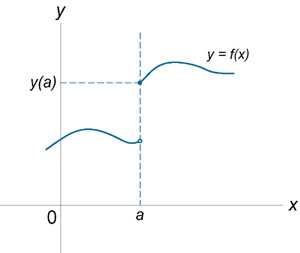
\includegraphics{img/fig1.jpg}
% \caption{Discontinuity}
% \end{figure}

% У заключения нет номера главы
\section*{Conclusion and future work}

\setmonofont[Mapping=tex-text]{CMU Typewriter Text}
% \bibliographystyle{plain}
% \bibliography{thesis}
\printbibliography
\end{document}
